\chapter{Anwendungsfall}
Im Rahmen dieser Arbeit wird die Verwendung von \gls{dp} Frameworks evaluiert und dazu eine prototypische Schnittstelle implementiert. Das folgende Kapitel führt einen konkreten Anwendungsfall für die drei Frameworks auf, wobei auf eine Anwendung in der medizinischen Forschung eingegangen wird. Anschließend wird der Ursprung der generierten Daten erläutert.
\section{Geplante Forschungsdatennutzung in der ePa}
Alle gesetzlich Versicherten können seit dem 1. Januar 2021 eine elektronische Patientenakte (\gls{ePa}) ihrer Krankenkassen erhalten \parencite{BGMePa}. In dieser werden medizinische Befunde, Informationen aus vorhergehenden Untersuchungen und Behandlungen über Praxis- und Krankenhausgrenzen hinweg umfangreich gespeichert. Der Patient kann durch verschiedene Endgeräte in einer dazugehörigen App seine medizinischen Unterlagen digitalisieren und in der \gls{ePa} abspeichern. Diese Daten liegen dann verschlüsselt darin vor. Die Daten werden nicht nur lokal verschlüsselt gespeichert, sondern auch innerhalb einer Telematikinfrastruktur, die zur schnellen Kommunikation zwischen den medizinischen Beteiligten dient.  Wenn ein Patient einem Arzt Zugriff auf seine \gls{ePa} gewähren möchte, dann muss er sie durch seine elektronische Gesundheitskarte und seine persönliche Identifikationsnummer freischalten. Zudem benötigt der Arzt seine Identifikationsnummer auf seinem Heilberufsausweis, welche als ein zweiter Schlüssel zum Lesen der \gls{ePa} dient. Alleinig der Patient kann inhaltliche sowie zeitliche Zugangsbeschränkungen seiner Daten festlegen. In der ersten Version ab 2021 konnte der Patient einer dritten Person lediglich kompletten oder gar keinen Zugriff gewähren. vollkommenen oder gar keinen Zugriff zuweisen. Ab der Änderung (zweite Version) im Jahr 2022 ist das Konfigurieren individueller Zugriffsberechtigungen pro Dokument möglich. So kann ein Zahnarzt nur einen Bruchteil der \gls{ePa} seines Patienten lesen, ein Hausarzt hingegen die gesamten Dokumente. Für 2023 ist eine dritte Version angekündigt, bei der eine persönliche digitale Identität hinterlegt wird, eine Datenfreigabe für Forschungszweck möglich ist und weitere Funktionalitäten hinzukommen werden.

Nach dem eingeführten Patientendatenschutzgesetz können die Patienten mit der dritten Version der \gls{ePa} ihre Daten der Forschung freigeben, was als Datenspende bezeichnet wird. So können verschiedene Verbände wie der Bundesverband der Deutschen Industrie e.V. (BDI), Bundesverband Medizintechnologie (BVMed) und weitere auf diese medizinischen Daten zugreifen, um z. B. ihre Versorgungsforschung gezielter zu führen. Die Daten der Datenspender werden nach dem Patientendatenschutzgesetz auf zentralen deutschen Servern gespeichert. Sie unterliegen den europäischen Datenschutzbestimmungen.

Dieses geplante Vorhaben wird in der \cref{fig:useCase} abgebildet. Im linken Bereich wird das zuvor beschriebene Szenario für die dritte Version im Jahr 2023 veranschaulicht.

\section{Erweitertes Szenario durch DP}
In dieser Arbeit wird der Einsatz von Frameworks mit \gls{dp} Funktionen am Beispiel einer Forschungsschnittstelle
evaluiert. Dafür wird der Anwendungsfall um das folgende Szenario erweitert.
\begin{figure}[!htbp]
	\centering
	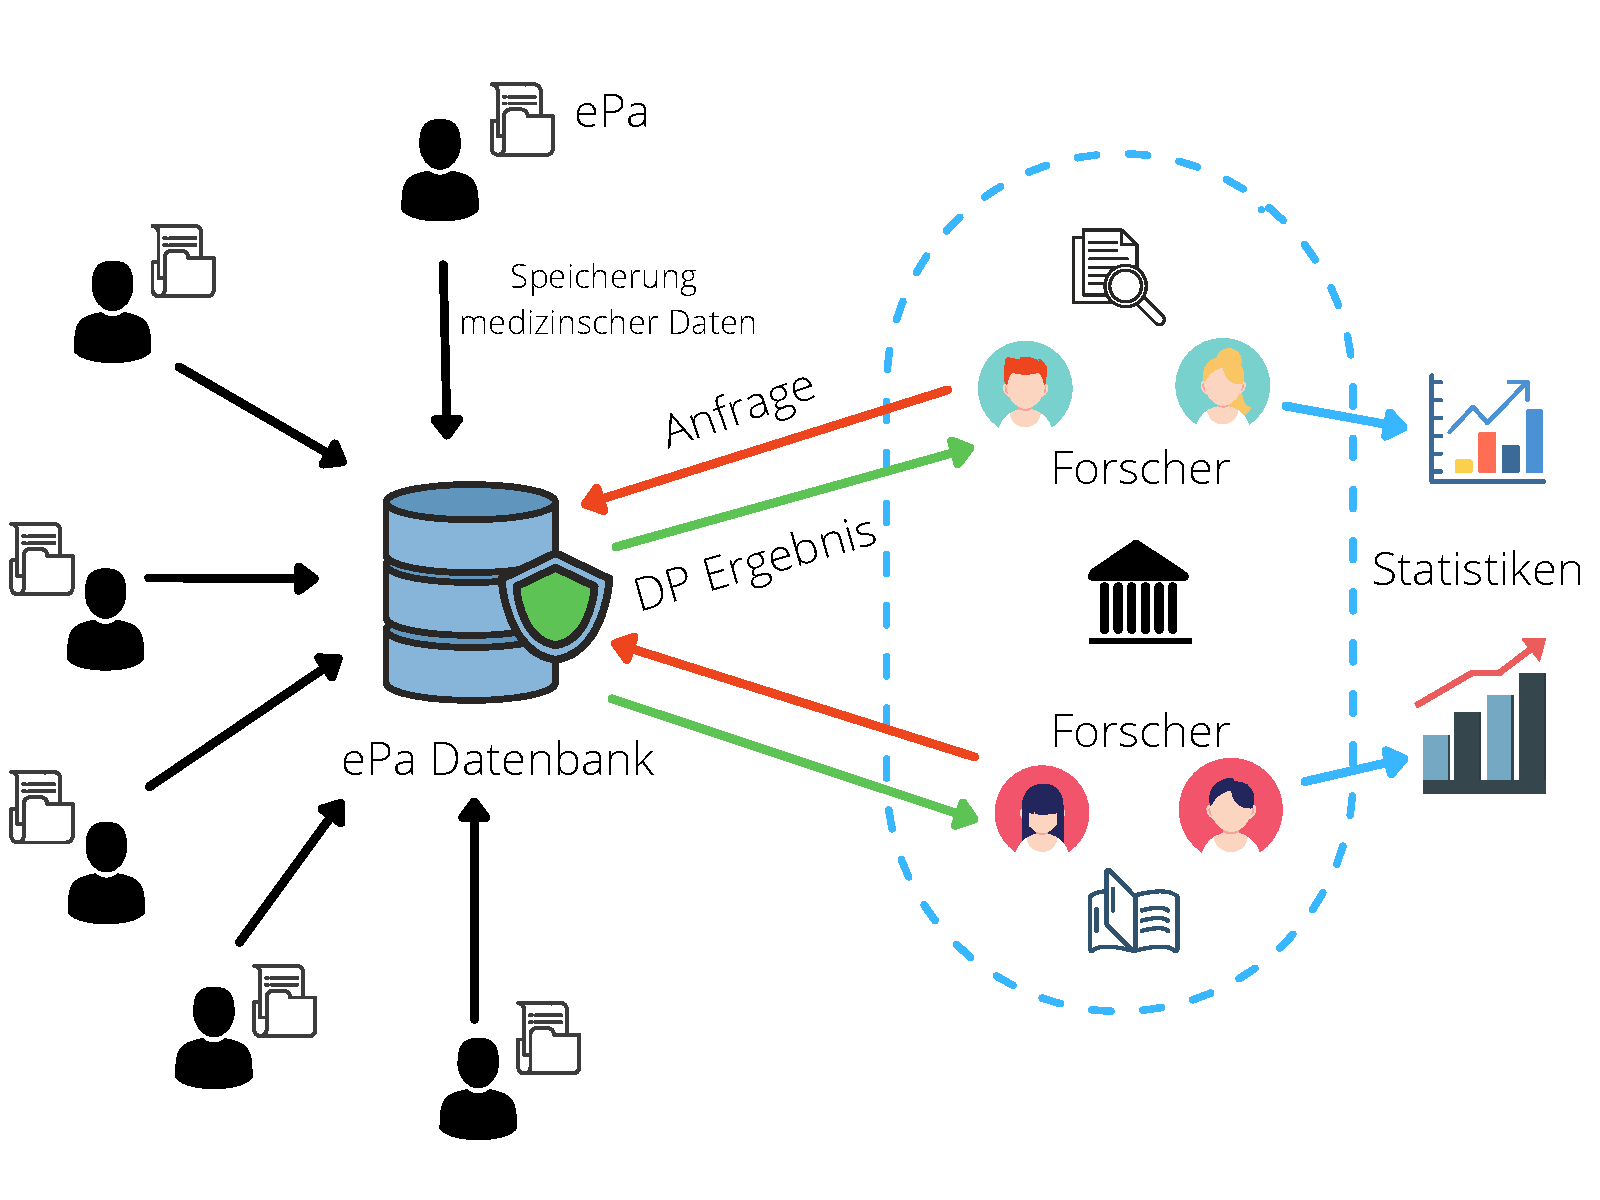
\includegraphics[scale=0.4]{./images/use_case.pdf}
	\caption{Die Visualisierung des Anwendungsfalls mit der Benutzung der \gls{ePa} und ihren dazugehörigen Akteuren.}
	\label{fig:useCase}
\end{figure}

Ein Forschungsinstitut stellt den Forschern ein Framework bereit, welches ein Zugriff unter der Bewahrung der Privatsphäre auf die \gls{ePa} Datenbank ermöglicht. In diesem Framework stellt ein Forscher eine Anfrage an die Datenbank. Das Framework verwertet die statistische Funktion der Anfrage unter Einhaltung von \gls{dp}, indem den Daten ein Rauschen hinzugefügt wird. Die hierfür benötigten Parameter des \gls{pb}s ist serverseitig festgelegt und nicht durch dritte Personen änderbar. Diese Parameter werden vom Staat in Einklang mit dem \gls{dsgvo} bestimmt und geändert (siehe Kapitel 1). Dieses verrauschte Ergebnis erhält der Forscher und verwendet es für seine Analysen und Statistiken. Anhand weiterer Anfragen können Zusammenhänge erkannt werden. Mit erfassten Kenntnisse können dann aussagekräftige Statistiken veröffentlicht werden. Hierbei wird nach der Definition von \gls{dp} die Beteiligung eines Patienten mit seiner \gls{ePa} nicht mehr ausschlaggebend, wodurch seine Privatsphäre geschützt wird.  

Dieses beschriebene Szenario dient als eine Weiterführung und wird in \cref{fig:useCase} im mittleren und rechten Bereich veranschaulicht.

\begin{figure}[htbp]
	\centering
	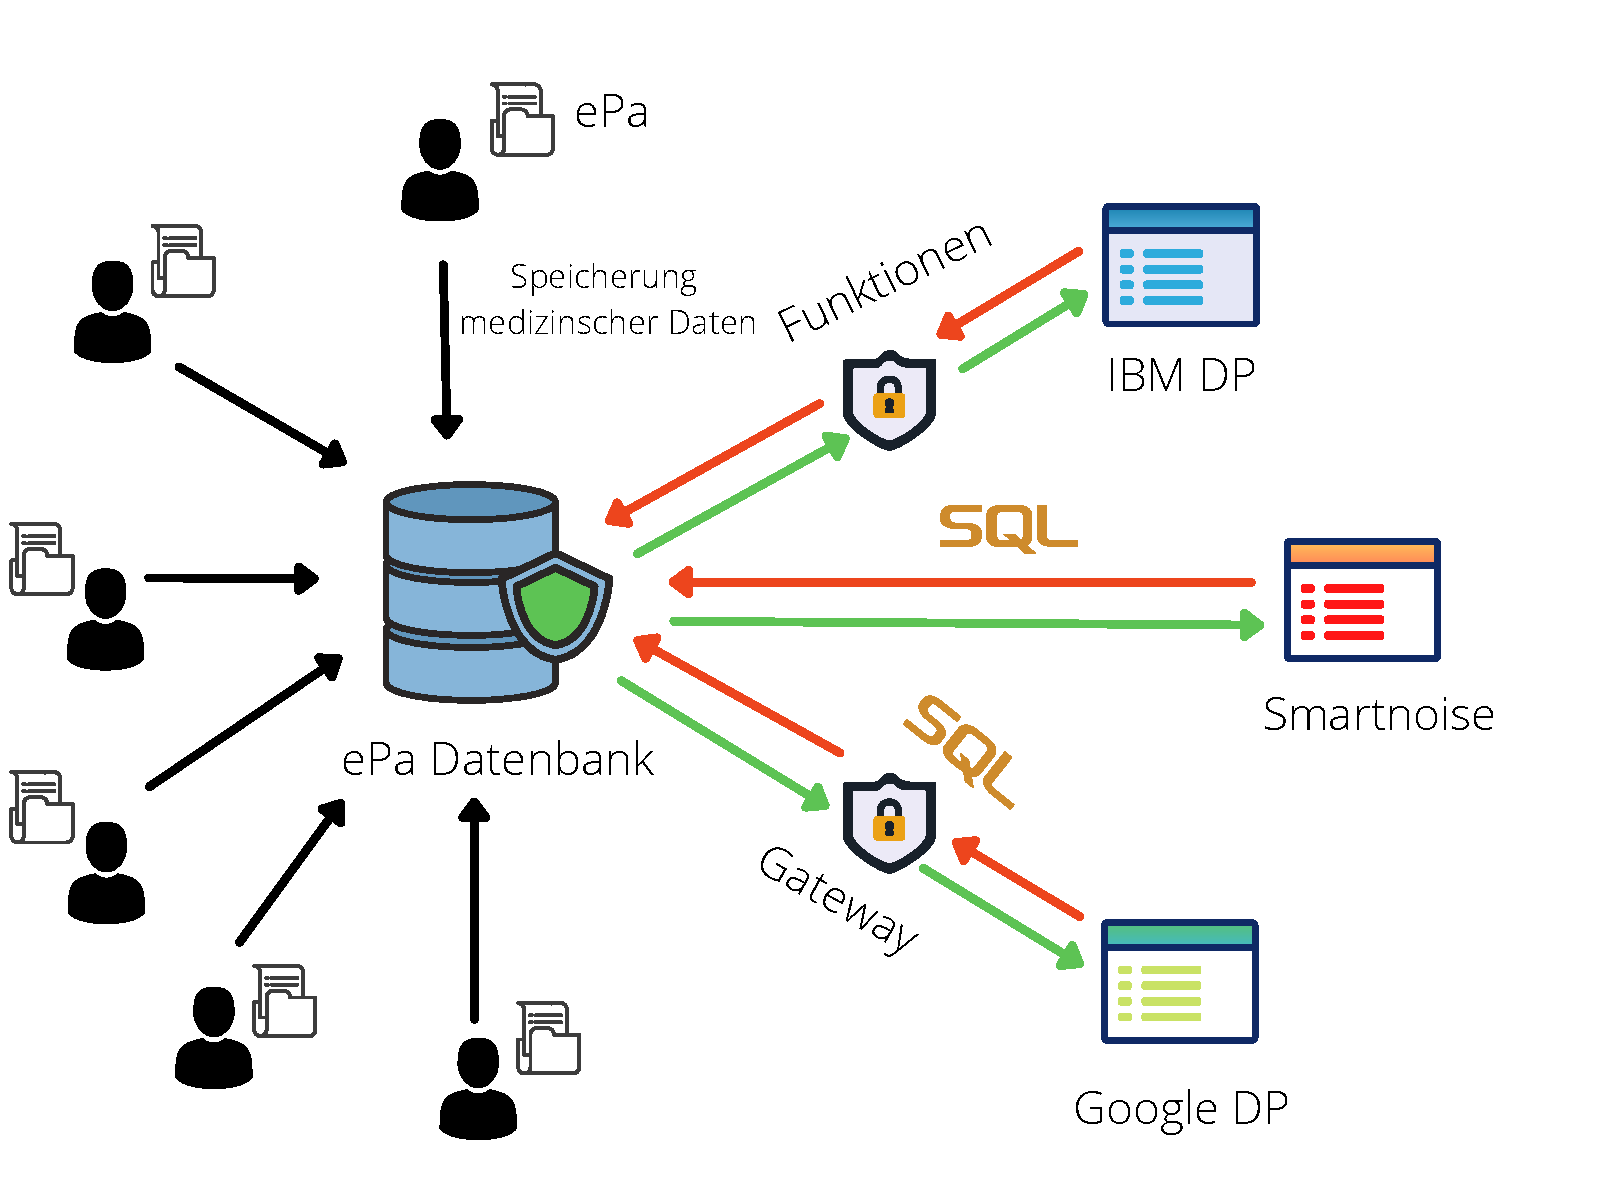
\includegraphics[scale=0.3]{./images/use_case2.pdf}
	\caption{Die Visualisierung des Anwendungsfalls mit der Benutzung der Frameworks.}
	\label{fig:use_case2}
\end{figure}

In Anbetracht des Szenarios kann eines der drei Frameworks eingesetzt werden. Der Einsatz eines jeweiligen Frameworks (IBM \gls{dp}, Smartnoise SDK und Google \gls{dp}) wird in der \cref{fig:use_case2} veranschaulicht. 
Das Smartnoise SDK Framework bietet zunächst die Verbindung zu einer Datenbank an. Aus dieser kann, ohne einen unmittelbaren Zugriff zu haben, Daten ausgelesen werden. Dagegen benötigen die Frameworks IBM \gls{dp} und Google \gls{dp} eine zusätzliche Verbindungsmöglichkeit zur Datenbank, denn sie können nur lokal Dateien auslesen. In den beiden Frameworks Smartnoise SDK und Google \gls{dp} werden die Anfragen durch die SQL-Sprache umgesetzt. Dabei werden die Parameter des \gls{pb}s durch den Forscher bestimmt, was dem Anwendungsfall widerspricht. Dies ist ebenfalls beim IBM \gls{dp} der Fall. Dieses Framework realisiert seine Anfragen anstatt durch die SQL-Sprache mit bereitgestellten statistischen Funktionen und \gls{ml} Modellen. Bei der Auswertung bietet dieses Framework noch zusätzlich die Generierung von verrauschten Histogrammen an. Dies kann in einer Statistik verwendet werden. Smartnoise SDK und Google \gls{dp} unterstützen explizit keine Funktionalitäten zur Visualisierung von Daten an, dagegen IBM \gls{dp} einige wenige wie z.B. verrauschte Histogramme.

\section{Rohdaten}
Für die Evaluation der Frameworks werden große Datenmengen benötigt. Diese sollen zu einem leicht verständlich sein und zugleich für den medizinischen Anwendungsfall geeignet sein. Dafür können synthetische Daten erzeugt oder bereits erfasste Daten im Gesundheitswesen genutzt werden. Für diese Bachelorarbeit wird ein hybrider Ansatz zwischen den beiden Möglichkeiten genommen. Zum einen wird eine CSV Datei vom \gls{rki} genutzt \parencite{RKIAltersverteilung}, welche die Anzahl an infizierten Patienten entsprechend der 19 Altersgruppen pro Kalenderwoche enthält. Für die Kalenderwochen 48 bis 52 (der Monat Dezember) wird die Wahrscheinlichkeitsverteilung der infizierten Personen pro Altersgruppe wie in \cref{tab : age_distribution} dargestellt, berechnet. Auf dieser Verteilung werden 1000 synthetisch generierte Werte für diese Altersgruppen erzeugt. Dieser Datensatz dient als Quelle für die Evaluation der Frameworks.

Zunächst wurde bei der Recherche ein großer Fokus auf Originaldaten im Bereich der Krankheit COVID-19 gesetzt. Verschiedene Institutionen und Länder haben Online-Portale sowie Datenbanken veröffentlicht, um die medizinischen Auswirkungen durch COVID-19 Krankheit in Zahlen auszudrücken

Dafür liegt ein großer Datenhub vom RKI vor, welcher die Covid-19 Infektionen pro 100.000 Einwohner der deutschen Bundesländern angibt \parencite{Datenhub}. Diese Statistik wird wöchentlich aktualisiert. Diese Datei mit tausenden Einträgen enthält genügend Informationen für die Evaluation und ist leicht durch eine CSV Datei einzulesen. Zusätzlich können die Anzahl der Attribute (Spalten) bestimmt werden. Jedoch sind die Daten zum einen inhaltlich teilweise schwierig zu verwenden, da sie schon privatisiert sind. Das Alter wird nur in Altersgruppen durch Kenneichungen angegeben und die Verteilung wird nach Bundesländern oder Landkreisen angeboten. Diese Problematik erschwert diese Datei als Basis der Evaluation zu verwenden.

Bei weiterer Recherche durch Kaggle, ein Online-Ansammlung von wissenschaftlichen Dokumenten, war eine Publikation des Landes Italien zur Krankheit COVID-19 sehr interessant \parencite{CovidItalien}. Hierbei handelt es sich um die Anzahl der Fälle sowie der Todesfälle nach Alter und Geschlecht für jede Region in Italien. Zwar ist die Datei an sich klein, jedoch können die darin enthaltenen Daten als Basis zur Synthese eines umfangreicheren Datensatzes genutzt werden. Das Ziel war für jedes Alter die spezifische Anzahl der Kranken zu erfassen. Aus Gründen der Privatsphäre wurden diese Daten schon privatisiert und nur in Altersgruppen veröffentlicht.
Nach weiterer Suche erfolgte der Fund desgleichen für Deutschland wie des von Italien, sodass dieser Datensatz für die Evaluation eingesetzt wird \parencite{RKIAltersverteilung}.
\begin{table}[ht]
	\centering
	\begin{tabular}{l l} \toprule
		\textbf{Altersgruppe} & \textbf{Wahrscheinlichkeit}  \\ \midrule
		0 - 4	&  4\% \\
		5 - 9	&  9\% \\
		10 - 14	&  10\% \\
		15 - 19	& 6\%  \\
		20 - 24	& 6\%  \\
		25 - 29	&  7\% \\
		30 - 34	&  8\% \\
		35 - 39	&  9\% \\
		40 - 44	&  8\% \\
		45 - 49	& 7\%  \\
		50 - 54	& 7\%  \\
		55 - 59	& 6\%  \\
		60 - 64	& 4.5\% \\
		65 - 69	&  3\% \\
		70 - 74	& 2\%  \\
		75 - 79	& 1\%  \\
		80 - 84	&  1,5\% \\
		85 - 89	& 0.5\%  \\
		90+& 0.5\%  \\ \bottomrule
	\end{tabular}
	\caption{Die Wahrscheinlichkeitsverteilung der COVID-19 infizierten Menschen nach den Altersgruppe im Dezember 2021.}
	\label{tab : age_distribution}
\end{table}
